\documentclass[a4paper]{article}
\usepackage[letterpaper, margin=1in]{geometry} % page format
\usepackage{listings} % this package is for including code
\usepackage{graphicx} % this package is for including figures
\usepackage{amsmath}  % this package is for math and matrices
\usepackage{amsfonts} % this package is for math fonts
\usepackage{hyperref} % for urls

\title{Homework 4}
\author{Morgan Baker}
\date{11/1/16}

\begin{document}
\lstset{language=Python}

\maketitle

\section{Question 1}
This was the only question on the assignment. The question was to use the k nearest neighbors algorithm to find the best Eout with a 10-fold Cross Validation. The dataset generator didn't work with the nearest negihbors algorithm because the data needed reshaping. The algorithm was finished and i got an array of Eouts that were only organized by their index, or the number of nearest neighbors/2 - 1. The output to this array can be seen in Figure \ref{fig:figure_3}. The remaining task was to create an algorithm to find the best eout, or the smallest number, and get the number of nearest neighbors that produced the value. I realized that some of the best k-values were produced from the first few iterations, which surprised me. With some of the other points, however, the algorithm  was definitely overfitting the data. The three best values, along with their n nearest neighbors, can be found in Figure \ref{fig:figure_1}. I ran this program a couple of times, and each time got similarresults. There would be one early index that did really well, and oine that did really well really late, but the third was usually a toss up. This honework was interesting because seeing this in action helped me learn something useful for my semester project, with finding different parts of numbers that can be recognized.
\begin{figure}
  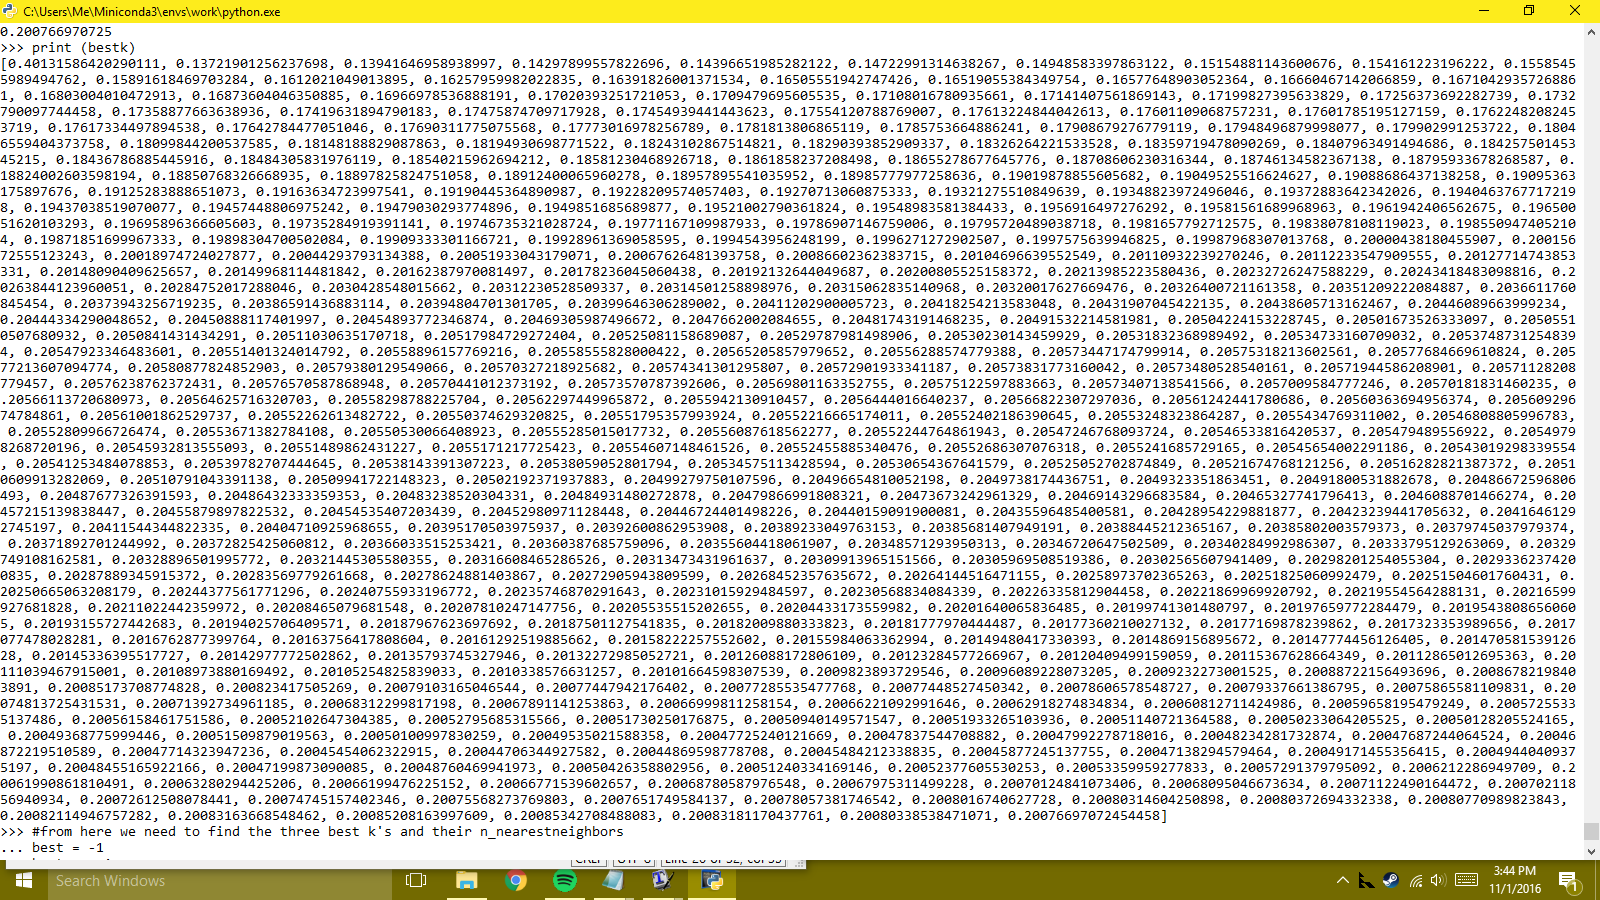
\includegraphics[width=\linewidth, height=9cm]{Eouts.png}
  \caption{The array of Eouts printed out to the console.}
  \label{fig:figure_3}
\end{figure}
\begin{figure}
  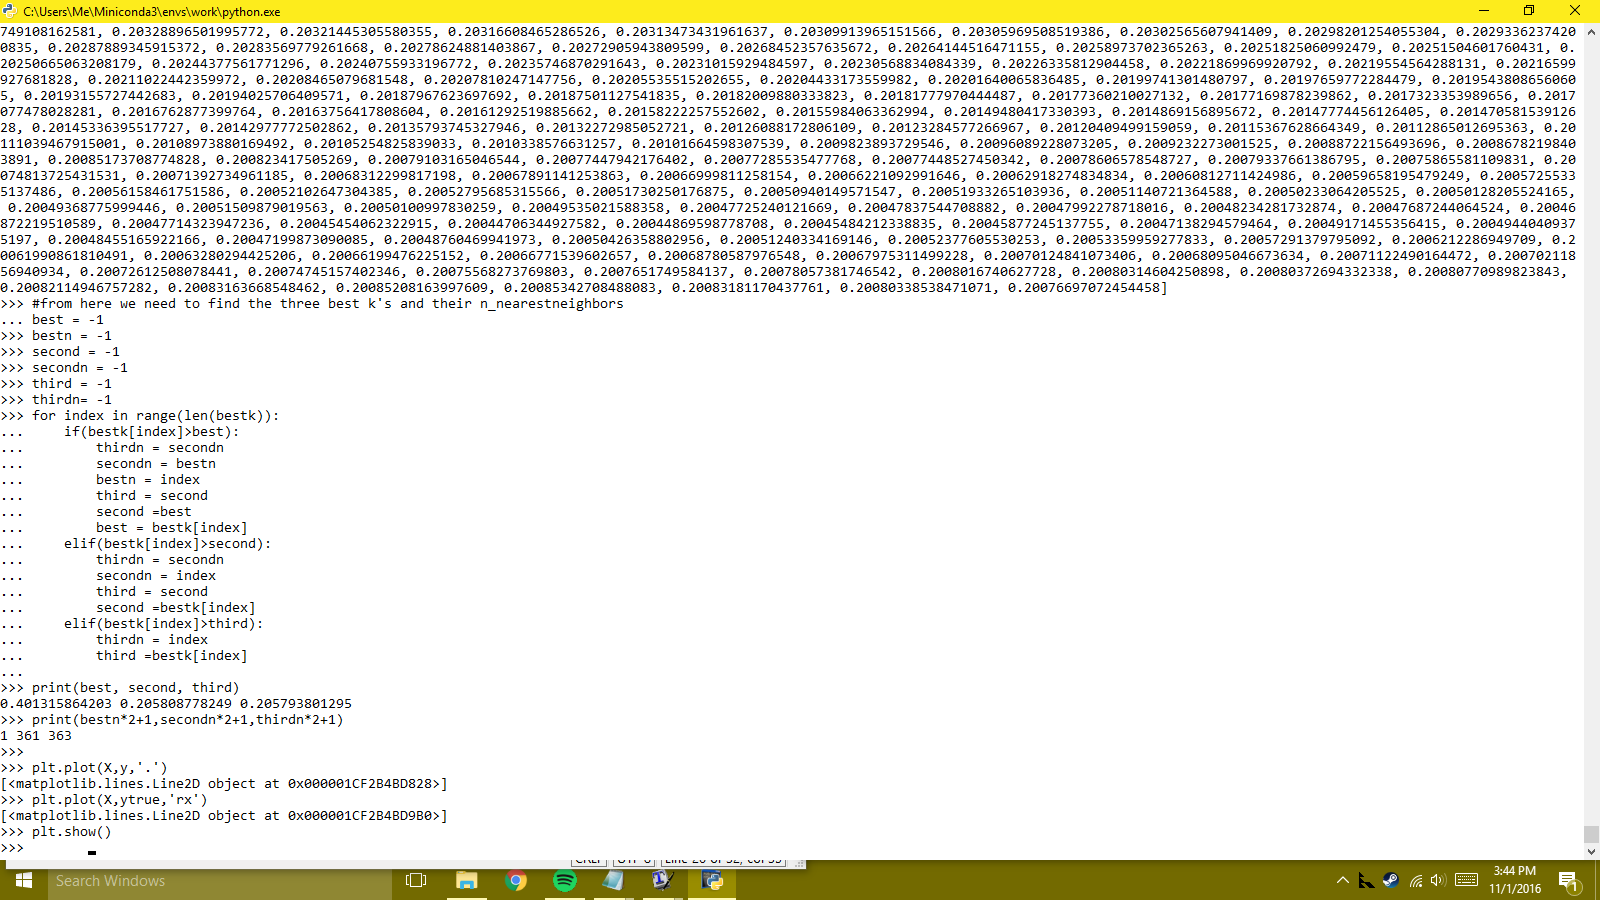
\includegraphics[width=\linewidth,height=9cm]{Best.png}
  \caption{The three best values of Eout, along with their number of nearest neighbors.}
  \label{fig:figure_1}
\end{figure}


\end{document}